% State of the Art

\chapter{State of the Art} % Main chapter title

\label{SoA} % For referencing the chapter elsewhere, use \ref{Chapter1} 

\lhead{Chapter 3. \emph{State of the Art}} % This is for the header on each page - perhaps a shortened title

This chapter provides an overview of the topics that supplied the ideas for this thesis. The
following sections examine the previous works which have been done on implementing
Visible Light Communication technology.

%----------------------------------------------------------------------------------------
%	VLC
%----------------------------------------------------------------------------------------

\section{VLC Implementations}

\subsection{Visible Light Communication System Considered}

An indoor visible light communication system using white LEDs under consideration is
shown in Fig. 3.1 and 3.2 [1]. All the lights in the room are replaced by LEDs. The LEDs
are not only used for illuminating the room but also for an optical wireless
communication system. On-off Keying Return-to-Zero (OOK-RZ) coding is used for
modulating white LEDs. Optical lighting and optical transmission of the white LEDs
have been tested to evaluate the requirements of using VLC for indoor applications. The
effects of the delay problems faced in the high data rate transmission have been studied
and presented [1].

Fig 3.1: VLC model room [1]. Fig 3.2: Distribution of LEDs inside model room [1].

\subsection{Visible Light Road-to-vehicle Communication Using High-Speed Camera}

LEDs are already being used in traffic lights, and they can be used as the communication
medium. Road-to vehicle communication using the LEDs in the traffic signal lights was
proposed.

Figure 3.3: Road-to-vehicle visible light communication [17].

The above Fig. 3.3 shows the basic usage of LED as a transmitter and CAMERA as a
receiver. In this model, they mounted a camera before the front end of the car. The
camera is used as the information receiver from traffic signal lights. The advantage of
using the camera is that multiple data can be transmitted by the LEDs and received by
High-speed cameras [17]. 


\subsection{Integrated System of White LED Visible-Light Communication and Power-Line Communication}

In [2], optical communication using the existing power-line in a household is proposed as
shown in \ref{fig:vlc-model}

\begin{figure}[htbp]
  \centering
    \scalebox{0.6}{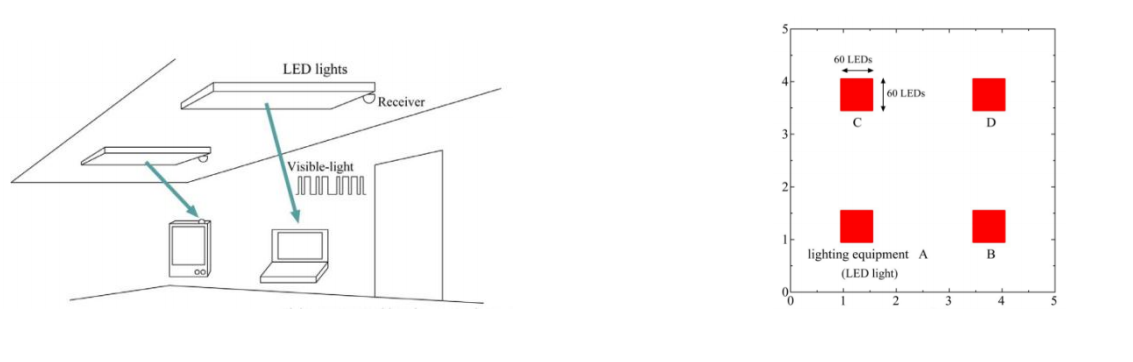
\includegraphics[width=\textwidth]{Pictures/vlc-model-room.png}}
    \rule{35em}{0.5pt}
  \caption[VLC System model]{VLC System model}
  \label{fig:vlc-model}
\end{figure}

The power-line is used for communication between white LEDs and other fixed
networks. The already installed power-lines and outlets behave as data networks and
ports.

\begin{figure}[htbp]
  \centering
    \scalebox{0.6}{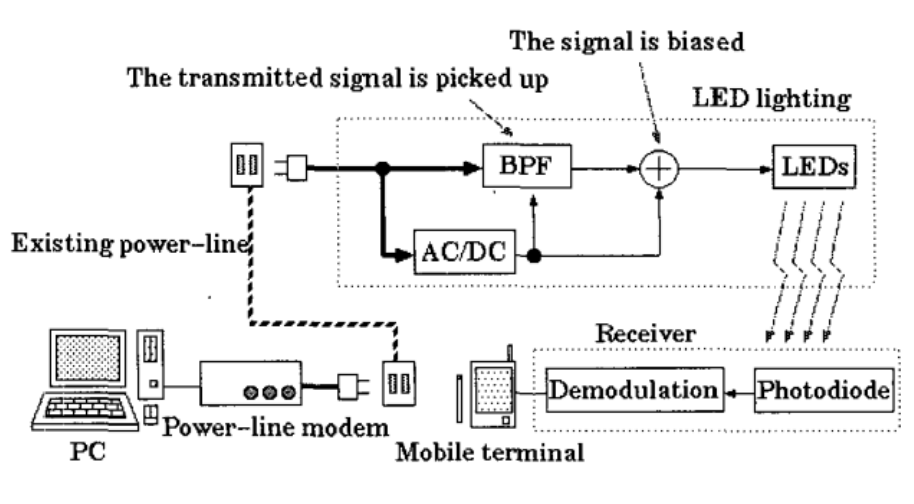
\includegraphics[width=\textwidth]{Pictures/vlc-powerline.png}}
    \rule{35em}{0.5pt}
  \caption[Waveform on power-linel]{Waveform on power-line}
  \label{fig:vlc-powerline}
\end{figure}

As in optical intensity modulation, the transmitted signals are added to the cyclic
waveform of the alternating current (AC). The transmitter signal from the PC is picked
by BPF through the power-line, and biased before sending to the LED lights. The
electrical signal is then converted into an optical signal by LEDs and sends it to the
photodiode, where it converts the captured optical signal to an electrical signal. The
signal is demodulated according to the received level of light and then is passed to the
mobile terminal [2].

\subsection{Visible Light Communication for Advanced Driver Assistant Systems}

\begin{figure}[htbp]
  \centering
    \scalebox{0.6}{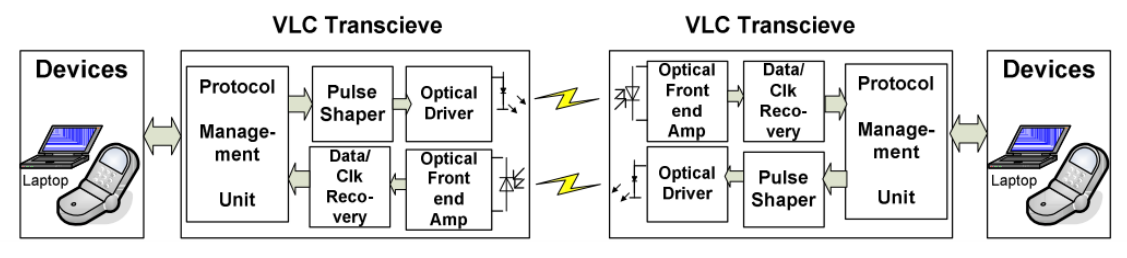
\includegraphics[width=\textwidth]{Pictures/vlc-driver.png}}
    \rule{35em}{0.5pt}
  \caption[General architecture for a full duplex VLC system ]{General architecture for a full duplex VLC system }
  \label{fig:vlc-driver}
\end{figure}

Optical communications for outdoor communication has been discussed and elaborated
upon [4]. Devices such as laptops and mobile phones can be used for transmitting and
receiving information, using transceivers, as shown in \ref{fig:vlc-driver}. Transceiver systems use
both LEDs and photodiodes. Intensity modulation was implemented to reach the most
viable modulation. Various important design parameters were optimized by using
intensive investigation based on gain variation over 100m of transmission range [4]. 


\subsection{Dual-Use Visible Light Approach to Integrated}

Communication and Localization of Underwater Robots with
Application to NonDestructive Nuclear Reactor Inspection
A VLC system for wireless underwater communication was proposed in [23] for robotic
inspection of nuclear power plants; there the reactor exists in an underground
environment as shown in Fig. 3.7. A solution for maintaining the consistent line of sight
to maintain a communication link was discussed in detail in [23].

Figure 3.7: Architecture of the dual-use optical communication system [23].

An optical wireless link has been established between the Remotely Operated Vehicles
(ROV) and gateway station using LEDs and Photodiodes on both sides as depicted in Fig
3.7. Underwater ROV was used to communicate with the gateway station over water to
transmit control signals. Both the gateway station and ROV are capable of directing a
light beam in the three-dimensional space [23]. 


\subsection{Study of Visible Light Communication System Using RGB LED Lights}

Figure 3.8: Outline of the system [24].

A prototype was designed to demonstrate wireless VLC using RGB LEDs and sensors
[24]. As shown in Fig. 3.8, on the left are the RGB LEDs used as signal transmitters. The
right side is the RGB sensor, which is used as a receiver. The RGB LEDs enable parallel
signal communication, and a PSoC microcontroller is used to control them, thus
significantly reducing the need for extra circuits. Pulse Width Modulation was used to
switch RGB LEDs at high speeds. The characteristics of both the variation in color and
change in intensity of each RGB LED and RGB sensor were analyzed to realize multiplevalue
signals communication by using RGB color [24]. 

\subsection{Visible Light Communication Link for Audio and Video Transmission}

Figure 3.9: Block diagram of transmitter module [27].
Figure 3.10: Block diagram of receiver module [27].
A VLC system to transmit high quality video and audio signal was proposed and
demonstrated by using illumination LEDs in [27]. The analog video signal was
modulated by using an ultra high speed comparator in the transmitter. The analog signal
was converted from analog to digital. Both the video and analog signals were transmitted
using the illumination LEDs in the transmitter. The photodiode at the receiver senses the
optical signals from the LEDs and is converted into electrical signals. The electrical
signal is then amplified to recover the digital signal and converted back to an analog
signal to video/ audio out [27]. 

\subsection{Ultra Thin Secondary Lens for Visible Light Communication Based on a White LED}
Figure 3.11: VLC system using WLED for personnel mobile telecommunication device
[42].
A new design was proposed in [42] for an ultra-thin secondary lens by using white
Surface Mount Device (SMD) LEDs for VLC. The GaN-based blue LEDs are used as
SMD LEDs and were mounted directly on the surface of the mobile device. The SMD
LEDs are used for optical transmission between mobile devices. The precise modeling of
the GaN chip was analyzed and verified. The modeling data were compared with
measured data to verify the proposed model. 


%----------------------------------------------------------------------------------------
%	SMARTPHONE SOLUTIONS
%----------------------------------------------------------------------------------------

\section{Smartphone solutions}

\subsection{Camera}
\subsection{External peripheral}

%----------------------------------------------------------------------------------------
%	CURRENT RESEARCHES
%----------------------------------------------------------------------------------------

\section{Current researches}